\title{CV Andrea Donadello}
\author{Andrea Donadello}

\documentclass[a4paper,11pt]{article}

\usepackage[T1]{fontenc}
\usepackage[empty]{fullpage}
\usepackage{titlesec}
\usepackage{marvosym}
\usepackage{verbatim}
\usepackage{enumitem}
\usepackage[hidelinks]{hyperref}
\usepackage{fancyhdr}
\usepackage{tabularx}
\usepackage{soul}
\usepackage{microtype}
\usepackage{graphicx}
% \usepackage[pass,showframe]{geometry}
\usepackage[a4paper, margin=1cm]{geometry}
\usepackage{tikz}

\input{glyphtounicode}

\pagestyle{fancy}
\fancyhf{} 

\setlength{\footskip}{12pt}

\renewcommand{\headrulewidth}{0pt}
\renewcommand{\footrulewidth}{0pt}

\setul{3pt}{0.5pt}

% Sections formatting
\titleformat{\section}{
  \vspace{-4pt}\scshape\raggedright\large
}{}{0em}{}[\color{black}\titlerule \vspace{-5pt}]
% Ensure that generate pdf is machine readable/ATS parsable
\pdfgentounicode=1

\graphicspath{{images/}}

%-------------------------
% Custom commands

\newcommand{\lefttabmargin}{0.025in}

\newcommand{\resumeItem}[1]{%
    \item\small{
        \begin{minipage}[t]{0.92\textwidth} 
            #1
        \end{minipage}
        \vspace{-2pt}
    }
}
\newcommand{\resumeSubheading}[4]{
  \vspace{-2pt}\item
    \begin{tabularx}{\textwidth}[t]{l@{\extracolsep{\fill}}r}
      \textbf{#1} & #2 \\
      \textit{\small#3} & \textit{\small #4} \\
    \end{tabularx}\vspace{-7pt}
}

\newcommand{\resumeSubSubheading}[2]{
    \item
        \begin{tabularx}{\textwidth}{@{\hspace{\lefttabmargin}}l@{\extracolsep{\fill}}r}
            \textit{\small #1} & \textit{\small #2} \\
        \end{tabularx}
}

\newcommand{\resumeProjectHeading}[3]{
    \item\begin{tabularx}{\textwidth}{@{\hspace{\lefttabmargin}}l@{\extracolsep{\fill}}r}
            \textbf{\large #1}  $|$  \small\textit{#2} & \small #3 \\
        \end{tabularx}\vspace{-7pt}
}

\newcommand{\resumeSubItem}[1]{\resumeItem{#1}\vspace{-4pt}}

\newcommand{\resumeSubHeadingListStart}{\begin{itemize}[leftmargin=\lefttabmargin, label={}]}
\newcommand{\resumeSubHeadingListEnd}{\end{itemize}}
\newcommand{\resumeItemListStart}{\begin{itemize}[label={\tiny$\bullet$}]}
\newcommand{\resumeItemListEnd}{\end{itemize}\vspace{-5pt}}

%-------------------------------------------

\begin{document}

\begin{minipage}{0.6\textwidth}
    \textbf{\huge Andrea Donadello} \vspace{0.3cm} \\
    Jesolo - Venice (Italy) \\
    April 28, 2000 \vspace{0.3cm} \\  
    \href{mailto:andreadonadello@outlook.com}{\ul{andreadonadello@outlook.com}} \\
    \href{https://linkedin.com/in/andreadonadello}{\ul{linkedin.com/in/andreadonadello}} |
    \href{https://github.com/adonadello}{\ul{github.com/adonadello}} \\
\end{minipage}
\hfill
\begin{minipage}{0.3\textwidth}
    \raggedleft
    \begin{tikzpicture}
        \clip (0,0)  circle (1.5cm) ;
        \node[anchor=center] at (0,0) {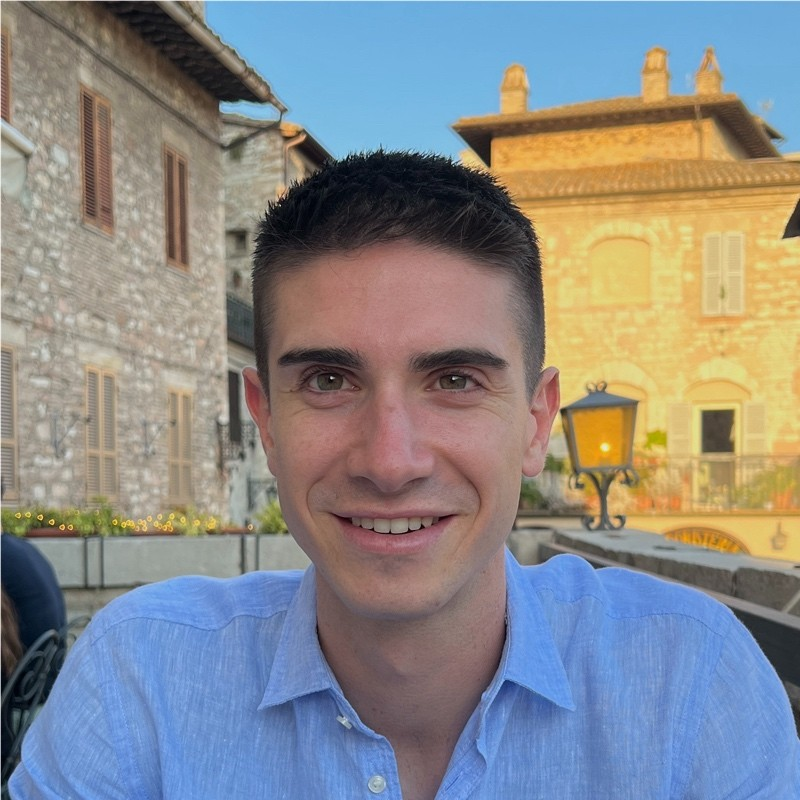
\includegraphics[width=3cm]{profile_photo.jpg}}; 
        %adjust this coordinate to move image
        \end{tikzpicture}
    \raggedleft
\end{minipage}
\noindent

%-----------EDUCATION-----------
\section{Education}
    \resumeSubHeadingListStart

        \resumeSubheading
            {Master's Degree in Big Data (Computer Engineering)}
            {Jun. 2024 - Present}
            {International Telematic UniNettuno University}
            {Rome, Italy}
        \resumeSubheading
            {Bachelor's Degree in Computer Engineering}
            {Jan. 2020 - Mar. 2024}
            {International Telematic UniNettuno University}
            {Rome, Italy}

    \resumeSubHeadingListEnd

%-----------EXPERIENCE-----------
\section{Experience}
    \resumeSubHeadingListStart

        \resumeSubheading{Software Backend Engineer}{June 2022 - Present}{Mediacy Srl}{Venice, Italy}
            \resumeItemListStart
                    \resumeItem{Developed and deployed web applications with Microservices Architecture and asynchronous routines.}
                    \resumeItem{Proficient in Java for backend development.}
                    \resumeItem{Integrated backend services with SpringBoot, focusing on configuration, optimization, and scalability.}
                    \resumeItem{Designed and optimized schemas and queries for PostgreSQL and Oracle databases.}
                    \resumeItem{Utilized Docker containers for application deployment, enhancing portability and scalability.}
                    \resumeItem{Configured and optimized Tomcat and WildFly web servers for Java applications.}    
            \resumeItemListEnd
        
    \resumeSubHeadingListEnd
    
%-----------PROJECTS-----------
\section{Projects}
    \resumeSubHeadingListStart

        \resumeProjectHeading{Backend Projects}{Java, SpringBoot, PostgreSQL, Oracle, Tomcat, Wildfly}{June 2022 -- Present}
            \resumeItemListStart
                \resumeItem{Utilized SpringBoot to develop efficient Java-based backend applications.}
                \resumeItem{Built RESTful APIs and microservices with SpringBoot for smooth inter-component communication.}
                \resumeItem{Optimized and configured SpringBoot applications for enhanced performance and scalability.}
                \resumeItem{Designed RESTful APIs for seamless frontend-backend integration, following RESTful principles.}
            \resumeItemListEnd
        \resumeProjectHeading{\href{https://github.com/adonadello/thesis}{\ul{Machine Learning Pipeline}}}{Scala, Akka, Kafka, Spark, Hadoop}{November 2023}
            \resumeItemListStart
                \resumeItem{Engineered a scalable machine learning pipeline using Scala, incorporating Kafka for real-time data streaming.}
                \resumeItem{Implemented Apache Spark for large-scale data processing and Akka for efficient concurrent processing.}
                \resumeItem{Optimized data transformation and enrichment processes, enhancing overall data quality and processing efficiency.}
            \resumeItemListEnd
        
    \resumeSubHeadingListEnd

%-----------PROGRAMMING SKILLS-----------
\section{Technical Skills}
    \begin{itemize}[leftmargin=0.025in, label={}]
        \small{\item{
            \textbf{Languages:} Italian (Native), English (Professional) \\
            \textbf{Programming Languages:} Java (Expert), C, SQL (PostgreSQL, Oracle) \\
            \textbf{Technologies:} Docker, Git, Tomcat, Wildfly \\
            \textbf{Frameworks:} SpringBoot, Akka \\
            \textbf{Tools:} Apache Kafka, Apache Spark, Hadoop 
    }}
    \end{itemize}

%-------------------------------------------
\end{document}